\documentclass[11pt, a4paper]{article}

\usepackage[utf8]{inputenc}
\usepackage[T1]{fontenc}

\usepackage[margin=2.5cm]{geometry}
\usepackage{helvet}
\renewcommand{\familydefault}{\sfdefault}

\usepackage{float}

\usepackage{graphicx}
\usepackage{xcolor}
\usepackage{authblk}

% --- Custom Boxes ---
\usepackage[most]{tcolorbox}
\tcbuselibrary{listings}

\newtcblisting{terminalbox}{
    colback=black!85!white,
    coltext=white,
    colframe=black,
    boxrule=1pt,
    arc=4pt,
    listing only,
    listing options={
        basicstyle=\ttfamily\color{white},
        breaklines=true
    },
    top=5pt, bottom=5pt, left=10pt, right=10pt
}

\newtcolorbox{Note}{
    colback=blue!5!white,
    colframe=blue!75!black,
    fonttitle=\bfseries,
    title=Note,
    arc=4pt
}

\newtcolorbox{Warning}{
    colback=red!5!white,
    colframe=red!75!black,
    fonttitle=\bfseries,
    title=Warning,
    arc=4pt
}

\usepackage{hyperref}
\hypersetup{
    colorlinks=true,
    linkcolor=blue,
    filecolor=magenta,      
    urlcolor=blue,
    pdftitle={Quaint - User Manual},
    pdfpagemode=FullScreen,
}
\begin{document}

\begin{titlepage}
    \centering
    \vspace*{4cm}

    {\fontsize{40}{48}\selectfont \textbf{Quaint}\par}
    \vspace{1cm}

    {\huge Interactive Quantum Wavepacket Simulator\par}
    \vspace{0.5cm}
    {\Large \textbf{User Manual}\par}

    \vspace{3.5cm}

    {\Large
        Jacek Winiarczyk \quad
        Szymon Borowski \quad
        Franciszek Hansdorfer \\[0.5em]
        Bartosz Łakomy \quad
        Adam Podkowiński
        \par}

    \vspace{1.5cm}

    {\large Faculty of Physics, University of Warsaw\par}
    \vspace{1cm}
    {\normalsize \textit{This project was developed under the mentorship of mgr Bartosz Kasza}\par}

    \vfill

    {\large \today\par}
\end{titlepage}

\newpage

\tableofcontents

\newpage

\section{Installation}
Quaint requires Python 3.10 or newer. To ensure a smooth installation of all dependencies, we strongly recommend using \texttt{uv}, a lightning-fast Python package installer and environment manager.

\subsection{Basic Installation}
Open your terminal and execute the following commands step by step to clone the repository and launch the application:

\begin{itemize}
    \item Clone the repository:
          \begin{terminalbox}
              git clone https://github.com/your-username/quaint.git
          \end{terminalbox}

    \item Navigate to the project directory:
          \begin{terminalbox}
              cd quaint
          \end{terminalbox}

    \item Install dependencies and create a virtual environment:
          \begin{terminalbox}
              uv sync
          \end{terminalbox}

    \item Activate the virtual environment:
          \begin{terminalbox}
              source .venv/bin/activate
          \end{terminalbox}

    \item Run the application:
          \begin{terminalbox}
              python main.py
          \end{terminalbox}
\end{itemize}

\subsection{Linux Troubleshooting (Qt \& xcb errors)}
Quaint utilizes PyQt6 for its graphical user interface. On Linux distributions (such as Ubuntu, Mint, or Debian), standard installations often lack the low-level windowing libraries required by Qt.

If the application crashes on startup with an error mentioning \texttt{qt.qpa.plugin: Could not load the Qt platform plugin "xcb"}, you need to install the missing system libraries. Run the following command to install the most common PyQt6 dependencies:

\begin{terminalbox}
    sudo apt update
\end{terminalbox}
\begin{terminalbox}
    sudo apt install libxcb-cursor0 libxkbcommon-x11-0 \textbackslash
    libxcb-xinerama0 libxcb-icccm4 \textbackslash
    libxcb-image0 libxcb-keysyms1 \textbackslash
    libxcb-randr0 libxcb-render-util0 \textbackslash
    libxcb-shape0
\end{terminalbox}
After installation, try running \texttt{python main.py} again.

\section{Getting Started}
Running your first quantum simulation is straightforward:
\begin{enumerate}
    \item Launch Quaint. The main 3D visualization window will appear.
    \item Click the \textbf{Simulation Setup} button located at the bottom of the screen.
          \begin{figure}[H]
              \centering
              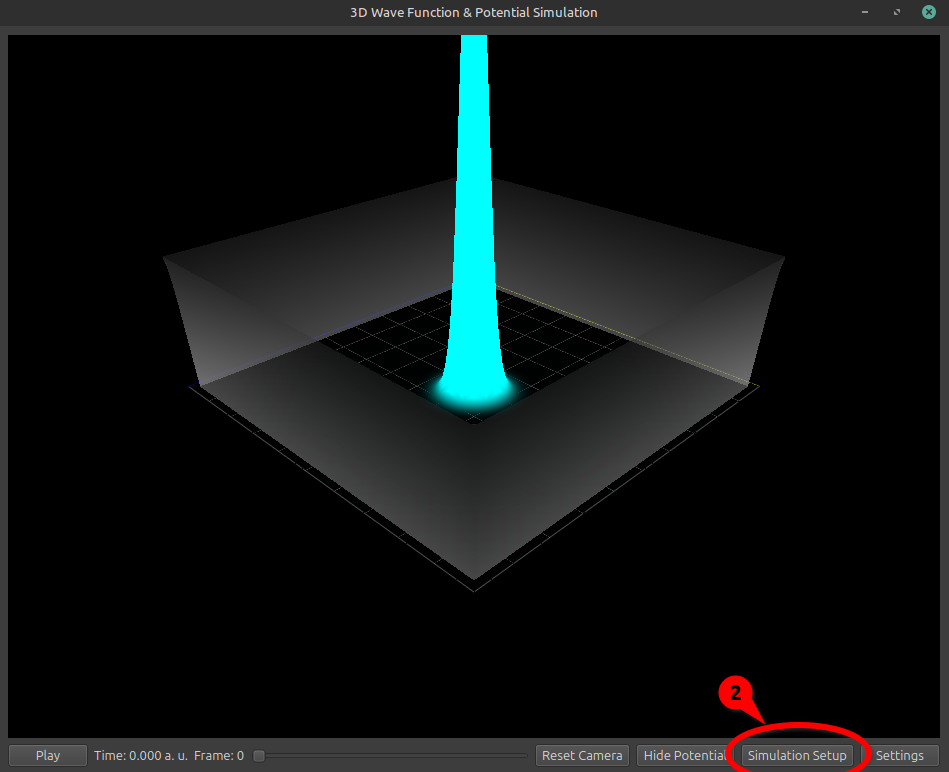
\includegraphics[width=0.7\textwidth]{images/step_2.png}
          \end{figure}
    \item In the right-hand panel of the setup window, locate the \textbf{Load Preset Potential} dropdown. Select \textit{Harmonic Oscillator}.
          \begin{figure}[H]
              \centering
              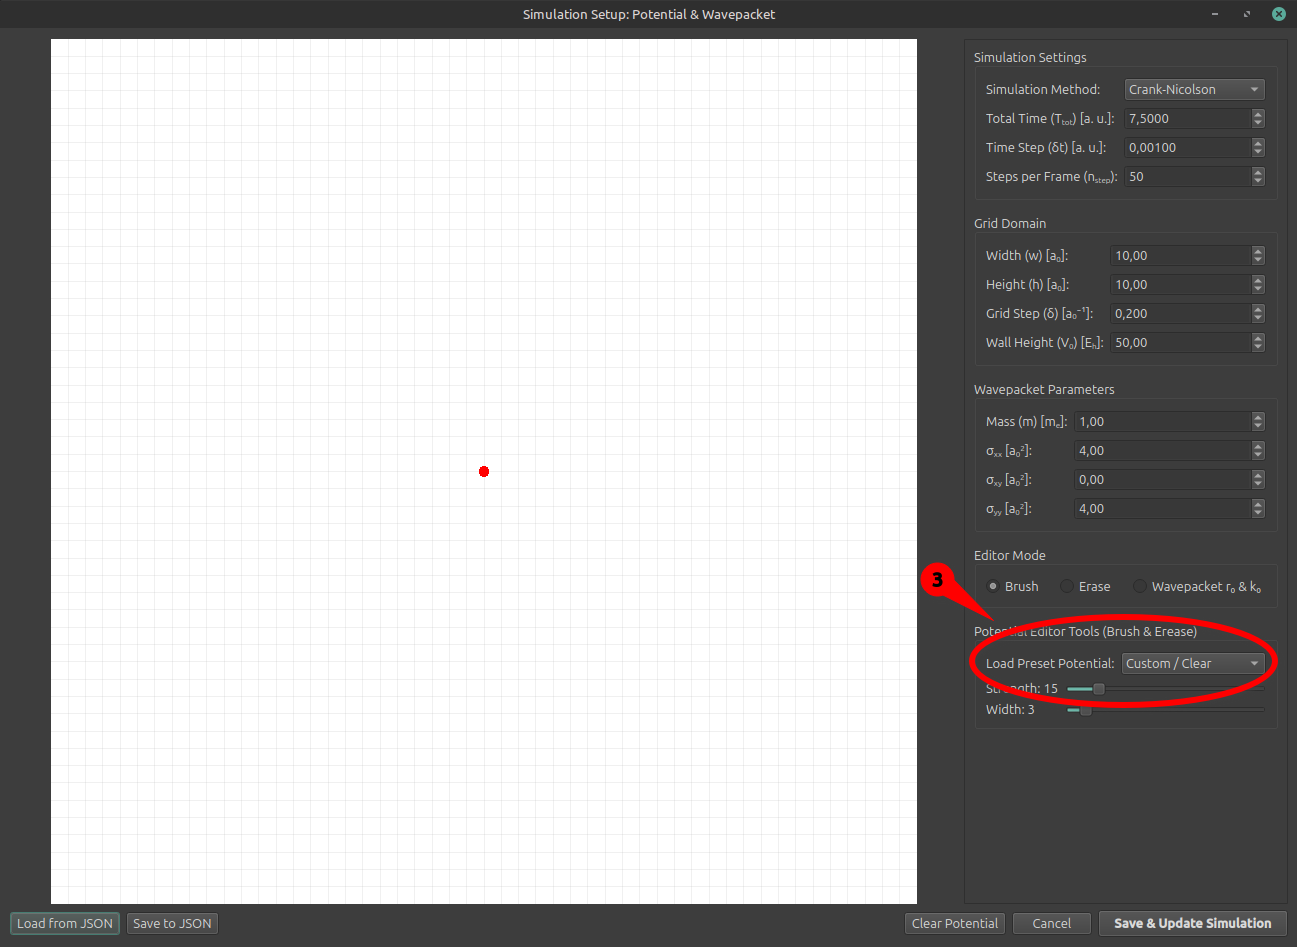
\includegraphics[width=0.7\textwidth]{images/step_3.png}
          \end{figure}
    \item Click \textbf{Save \& Update Simulation} at the bottom right.
          \begin{figure}[H]
              \centering
              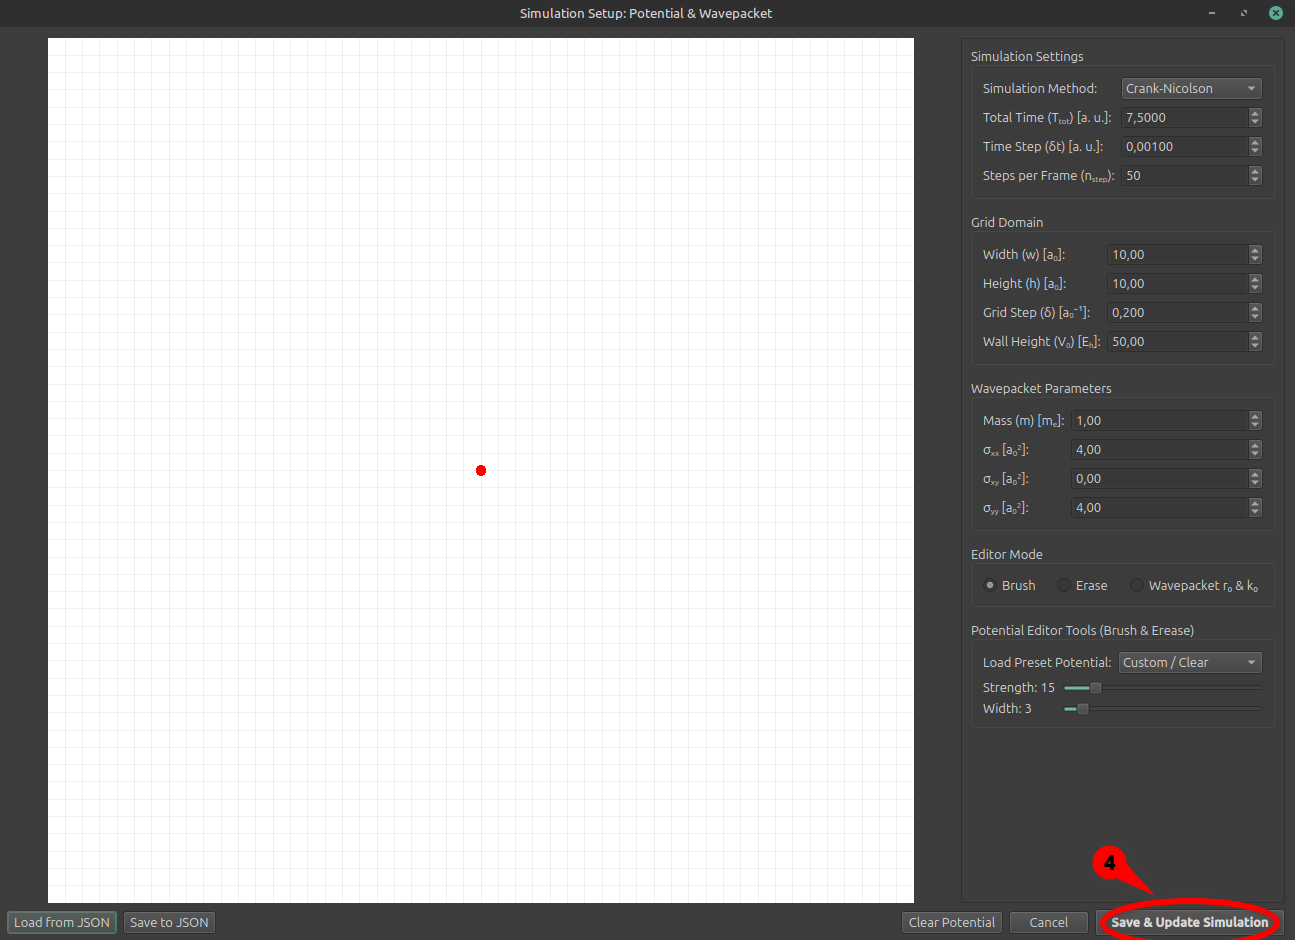
\includegraphics[width=0.7\textwidth]{images/step_4.png}
          \end{figure}
    \item Once the calculation is complete, press the \textbf{Play} button (or the Spacebar) to watch the wavepacket evolve in the potential well.
          \begin{figure}[H]
              \centering
              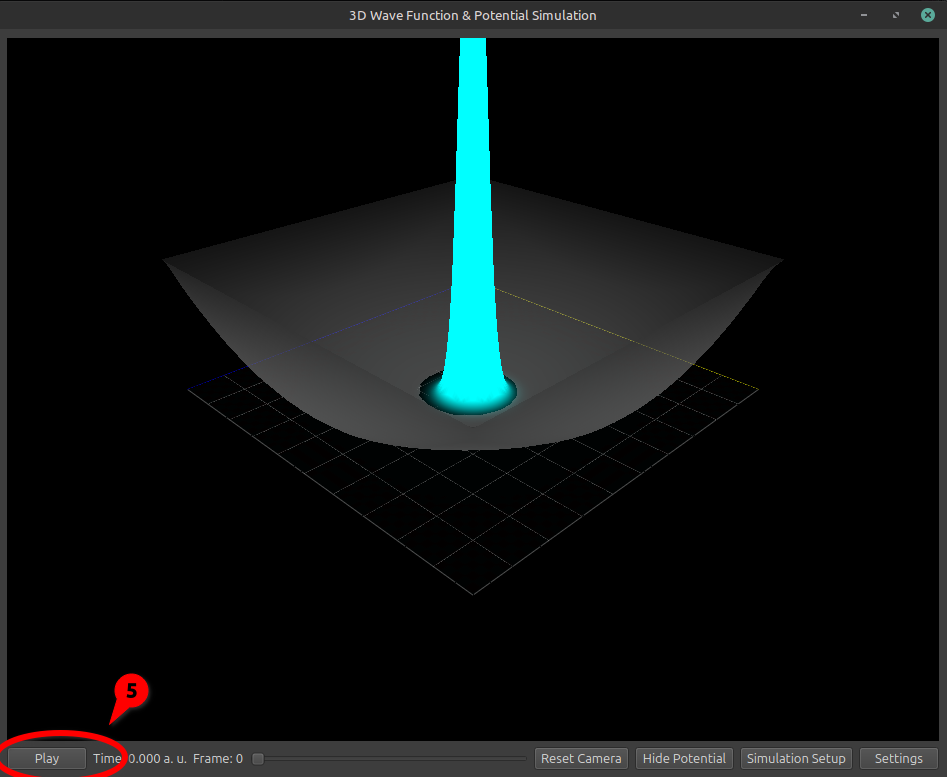
\includegraphics[width=0.7\textwidth]{images/step_5.png}
          \end{figure}
\end{enumerate}

\section{Animation Window}
The main window is dedicated to the real-time, 3D OpenGL visualization of the wavepacket and the underlying physical potential landscape.

\subsection{Camera Controls}
The simulation is rendered in full 3D space. You can navigate the view freely using your mouse:
\begin{itemize}
    \item \textbf{Rotate:} Left-click and drag the mouse across the canvas.
    \item \textbf{Zoom:} Right-click and drag (up/down) or use your mouse scroll wheel.
    \item \textbf{Pan:} Middle-click (scroll wheel click) and drag to move the camera focus point.
\end{itemize}

\subsection{Playback Controls}
Located at the bottom of the screen, the playback bar allows you to traverse the calculated simulation frames.

\begin{figure}[H]
    \centering
    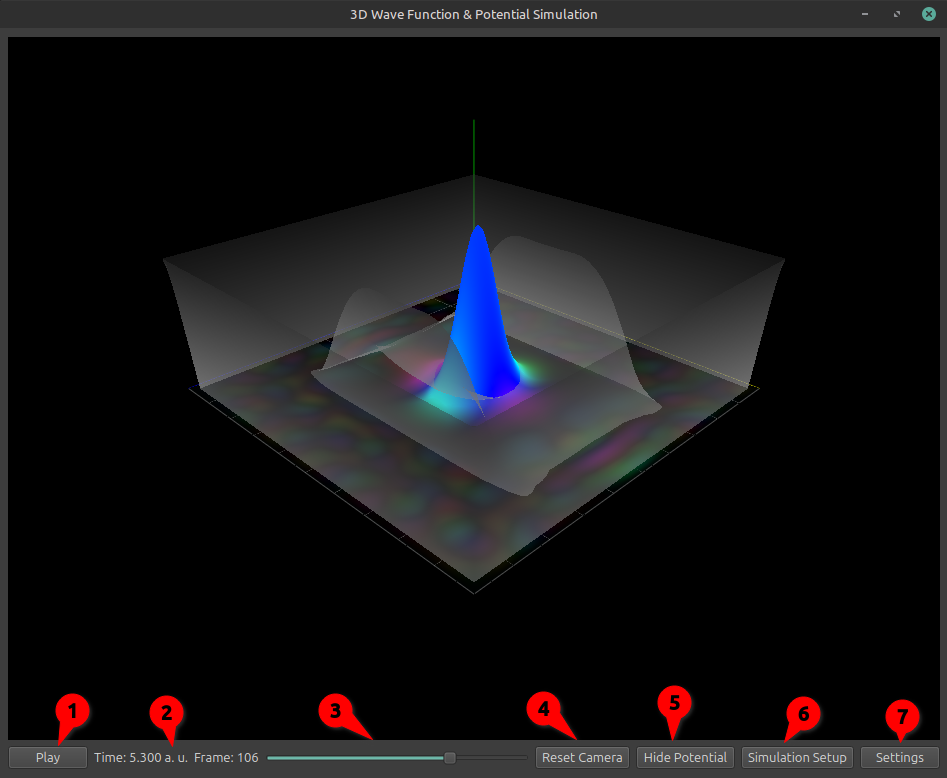
\includegraphics[width=0.7\textwidth]{images/animation_window.png}
    \caption{Main 3D animation window.}
\end{figure}

\begin{itemize}
    \item \textbf{Play / Pause (1):} Toggles the animation playback. Alternatively, you can use the \textbf{Spacebar} as a global shortcut.
    \item \textbf{Time Label (3):} Displays the current physical time elapsed in atomic units (a.u.) and the current frame index.
    \item \textbf{Timeline Slider (2):} Click and drag the slider to scrub through the animation manually.
    \item \textbf{Reset Camera (4):} Instantly snaps the 3D camera back to its default viewing angle and distance.
    \item \textbf{Hide / Show Potential (5):} Toggles the visibility of the semi-transparent 3D potential mesh. Hiding it can give you a clearer, unobstructed view of the complex wave function.
    \item \textbf{Simulation Setup (6):} Opens the setup drawer, pausing the simulation and allowing you to redefine physical parameters and the environment.
    \item \textbf{Settings (7):} Opens a dedicated window for visual configuration (e.g., rendering scales, brightness).
    \item \textbf{Stop Calculation:} This button only appears while the backend is computing a new simulation. Clicking it safely aborts the heavy calculation without crashing the program, allowing you to return to the setup window.
\end{itemize}

\begin{figure}[H]
    \centering
    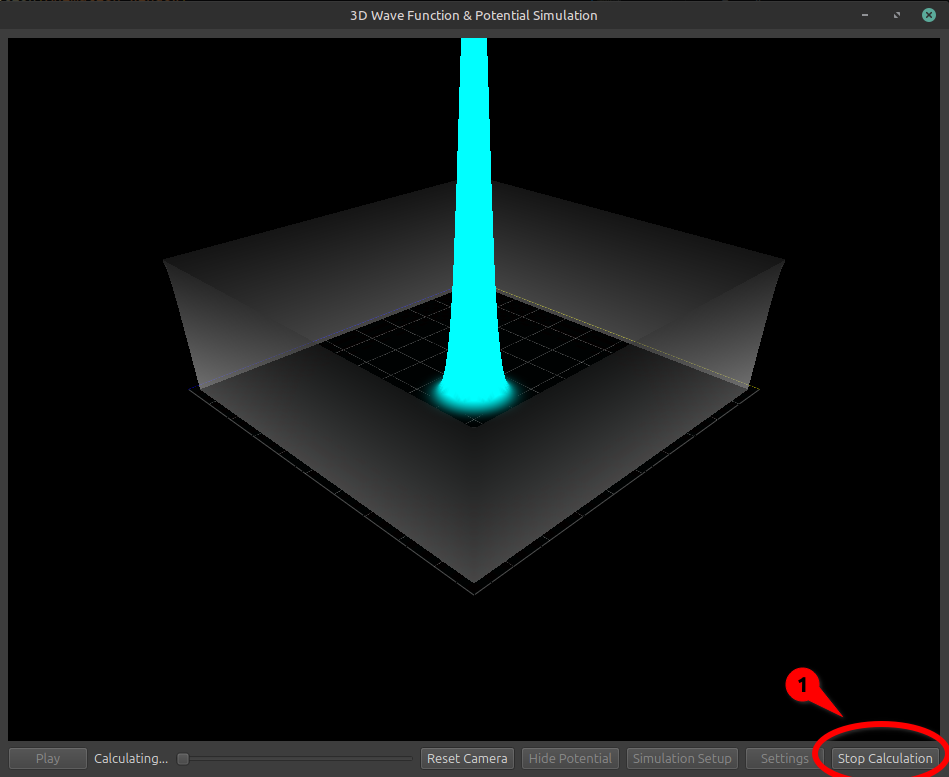
\includegraphics[width=0.7\textwidth]{images/calculating_mode.png}
    \caption{Main 3D animation window in calculation mode.}
\end{figure}

\section{Simulation Setup Window}
The Setup Drawer is the core of Quaint. It is a comprehensive physics configuration interface linking your manual drawings to the mathematical simulation parameters.

\begin{figure}[H]
    \centering
    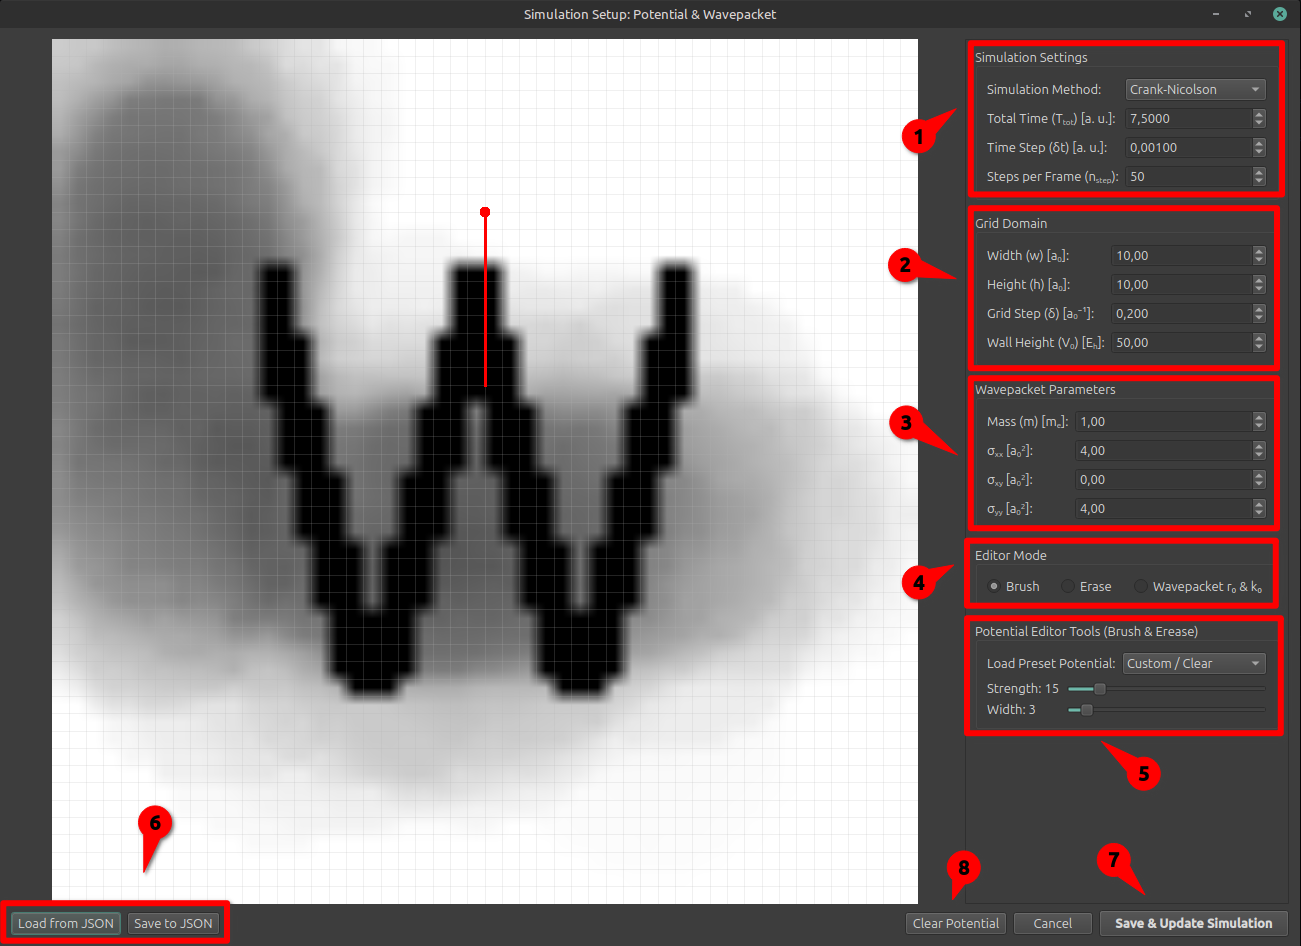
\includegraphics[width=0.7\textwidth]{images/setup_window.png}
    \caption{The Simulation Setup interface.}
\end{figure}

\subsection{Painting the Potential}
The left side of the window is an interactive canvas representing your 2D spatial grid.

\begin{Note}
    The simulation domain is strictly bounded by infinite potential walls. Any wavepacket reaching the edge of the canvas will reflect back. If you wish to simulate free space for a longer duration, you must increase the physical dimensions of the grid.
\end{Note}

You can modify the potential landscape using the \textbf{Editor Mode (4)} tools:
\begin{itemize}
    \item \textbf{Brush:} Click and drag to paint potential barriers.
    \item \textbf{Erase:} Click and drag to remove previously drawn potential barriers, resetting those specific grid cells to zero potential.
    \item \textbf{Wavepacket $r_0$ \& $k_0$:} Sets the initial state of the quantum particle. Click once on the canvas to anchor the initial position ($r_0$), then drag outward and release to define the initial momentum vector ($k_0$). The length and direction of the drawn arrow dictate the speed and trajectory of the packet.
\end{itemize}

To gain finer control over the drawing tools, adjust the sliders in the \textbf{Potential Editor Tools (5)} section:
\begin{itemize}
    \item \textbf{Strength Slider:} Adjusts the height of the drawn potential. A value of $100$ corresponds to the maximum wall height defined in your grid settings, while lower values create softer barriers.
    \item \textbf{Width Slider:} Changes the diameter of the brush (and eraser) in grid cells.
\end{itemize}

\subsection{Preset Potentials}
Instead of drawing by hand, you can automatically generate precise, mathematical potential landscapes using the \textbf{Load Preset Potential} dropdown from the \textbf{Potential Editor Tools (5)} section. Selecting any of the presets will immediately overwrite the canvas with the corresponding potential shape and reset the wavepacket to its default position for that scenario:
\begin{itemize}
    \item \textbf{Custom / Clear:} Wipes the canvas clean to a flat, zero-potential state.
    \item \textbf{Gaussian Bump:} Generates a smooth, central potential hill.
    \item \textbf{Harmonic Oscillator:} Creates a classic parabolic well originating from the center of the grid, with the wavepacket in the center by default.
    \item \textbf{W-shape:} Forms an intricate double-well potential structure. The preset automatically drops the wavepacket near the top center with a downward momentum.
    \item \textbf{Matryoshka:} Creates a scaled down version of the current canvas state in the center, surrounded by potential walls.
    \item \textbf{Slab:} A simple vertical barrier dividing the grid into two halves.
\end{itemize}

\subsection{Setup Options}
The right panel contains precise numerical parameters defining the physics engine behavior.

\subsubsection{Simulation Settings}
The \textbf{Simulation Settings (1)} section allows you to configure the core numerical parameters of the time evolution algorithm and the simulation method.
\begin{itemize}
    \item \textbf{Simulation Method:} Choose the numerical algorithm for time evolution. \textit{Crank-Nicolson} is unconditionally stable and highly accurate, but can be slower on very large grids. \textit{SSFM} (Split-Step Fourier Method) and \textit{Symmetric SSFM} are typically faster for large domains but require periodic boundaries.
    \item \textbf{Total Time ($T_{tot}$):} The total physical duration of the simulation in atomic units.
    \item \textbf{Time Step ($\delta t$):} The size of each mathematical integration step. Smaller values increase accuracy but require more calculations.
    \item \textbf{Steps per Frame ($n_{step}$):} The number of background simulation steps calculated before capturing a single frame for the animation. Increasing this speeds up the visual playback of long simulations without losing mathematical accuracy.
\end{itemize}

\begin{Warning}
    \textbf{Numerical Stability:} Quantum simulations are highly sensitive to initial conditions. If your Time Step ($\delta t$) is too large relative to the Grid Step ($\delta$), the numerical solver may diverge.

    Quaint features an automatic stability checker. Instead of crashing or producing broken "exploding" artifacts, Quaint will intercept unstable parameters, display a detailed warning, and safely return you to the Setup window so you can lower the time step or adjust the grid.

\end{Warning}

\begin{figure}[H]
    \centering
    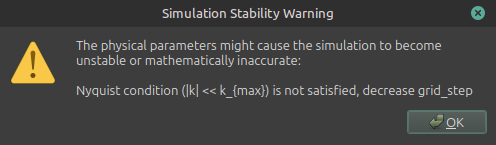
\includegraphics[width=0.6\textwidth]{images/stability_warning.png}
    \caption{A stability warning pop-up.}
\end{figure}

\subsubsection{Grid Domain}
The \textbf{Grid Domain (2)} parameters define the physical dimensions and resolution of your simulation space.
\begin{itemize}
    \item \textbf{Width ($w$) \& Height ($h$):} The physical dimensions of the simulation space, measured in Bohr radii ($a_0$).
    \item \textbf{Grid Step ($\delta$):} The distance between individual calculation nodes.

          \begin{Note}
              Smaller steps provide significantly higher spatial resolution, but exponentially increase memory usage and computation time. If your simulation takes too long to generate or the interface lags, increasing the Grid Step is the most effective way to speed it up.
          \end{Note}

    \item \textbf{Wall Height ($V_0$):} The maximum potential energy value in the simulation, measured in Hartrees ($E_h$). This value acts as the ceiling for your Brush tool.
\end{itemize}

\subsubsection{Wavepacket Parameters}
The \textbf{Wavepacket Parameters (3)} allow you to define the initial quantum state of the particle before time evolution begins. The wavepacket is mathematically represented as a 2D Gaussian function, and these parameters control its shape and spread.
\begin{itemize}
    \item \textbf{Mass ($m$):} The mass of the simulated particle, expressed in units of electron mass ($m_e$).
    \item \textbf{$\sigma_{xx}$ \& $\sigma_{yy}$:} The spatial uncertainty (spread) of the initial wavepacket along the X and Y axes, measured in squared Bohr radii ($a_0^2$). Larger values create a wider, more diffuse initial packet.
    \item \textbf{$\sigma_{xy}$:} The correlation between the X and Y uncertainties, allowing you to create diagonally skewed wavepackets.
\end{itemize}

\subsection{Saving and Loading Configurations}
Achieved a fascinating quantum simulation? You can preserve your setup using the buttons in the bottom left corner \textbf{(6)}.
\begin{itemize}
    \item \textbf{Save to JSON:} Exports your entire canvas drawing, potential height, and all physical parameters to a lightweight JSON file.
    \item \textbf{Load from JSON:} Imports a previously saved configuration, immediately overwriting the current canvas and settings.
\end{itemize}
Once you are satisfied with all parameters, click \textbf{Save \& Update Simulation (7)} to build the matrices and begin the heavy calculation process.

\section{Visual Settings}
Clicking the \textbf{Settings} button in the main window opens a non-modal dialog dedicated strictly to rendering aesthetics. Modifying these values updates the 3D view instantly \textit{without} forcing a simulation recalculation.

\begin{figure}[H]
    \centering
    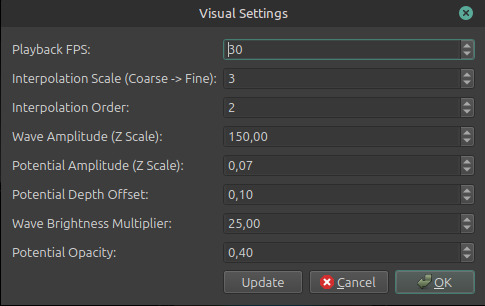
\includegraphics[width=0.7\textwidth]{images/settings_window.png}
    \caption{Visual settings dialog.}
\end{figure}

\begin{itemize}
    \item \textbf{Playback FPS:} Adjusts the target frames-per-second rate of the animation player.
    \item \textbf{Interpolation Scale:} The application renders the wave function on a visually finer grid than the one used for actual physics calculations. This value dictates how many visual cells correspond to one physical grid cell.
    \item \textbf{Interpolation Order:} Controls the B-spline math used during upscaling. Order 1 is fast but faceted; Order 2 is the recommended sweet spot; Order 3+ is very smooth but computationally heavier and might artificially overshoot near sharp peaks.
    \item \textbf{Wave Amplitude (Z Scale):} A purely visual multiplier that stretches the probability peaks upwards, making them easier to distinguish from the floor.
    \item \textbf{Potential Amplitude (Z Scale):} Vertically stretches the 3D potential mesh.
    \item \textbf{Potential Depth Offset:} Physically shifts the entire potential mesh up or down along the Z-axis to prevent it from clipping through the wave function.
    \item \textbf{Wave Brightness Multiplier:} Increases the color exposure of the wave graph. This is useful for visualizing extremely faint probability tails that have tunneled through barriers.
    \item \textbf{Potential Opacity:} Controls the transparency level (Alpha channel) of the potential landscape.
\end{itemize}

\end{document}